\documentclass[review,12pt]{elsarticle}

% ---- Chinese support (compile with XeLaTeX) ----
\usepackage{ctex}
\usepackage{graphicx}
\usepackage{booktabs}
\usepackage{amsmath,amssymb}
\usepackage{multirow}
\usepackage[hidelinks]{hyperref}
\graphicspath{{./}}

\journal{Information Fusion}

\begin{document}

\begin{frontmatter}

\title{异构大语言模型协作的反馈驱动自适应 DAG 执行：机制与适用边界
\\[6pt]
\large Feedback-Driven Adaptive DAG Execution for Heterogeneous Large Language Model
Collaboration: Mechanisms and Applicability Boundaries}

\author[inst1]{作者一\corref{cor1}}
\ead{author1@institution.edu}
\cortext[cor1]{通讯作者}
\author[inst1]{作者二}
\address[inst1]{单位，城市，国家}

\begin{abstract}
（中文摘要，与冻结稿逐字一致）复杂任务包含信息抽取、关系推理和结果验证等不同能力需求，针对完整查询选择单一模型难以利用执行阶段间的模型互补。本文提出反馈感知的自适应有向无环图路由框架，将能力画像、节点级模型分配、静态执行与反馈条件化的后继适应相结合，并以选择性干预、预算约束和历史图复用组织多模型协同。财务复杂任务实验表明，冻结节点路由相对查询路由的条件化节点质量提高约 6.9 个百分点，主要收益来自阶段粒度；严格配对的三臂分解基准（300 任务、一次统一会话）进一步表明，同模型拆分本身在 TAT-QA 上显著有害（−21.0pp）、在 MultiHiertt 上不显著，而拆分后的异构阶段分工带来总体 +5.0pp 的显著增益、但未完全抵消分解损耗——DAG 的核心作用是解除阶段能力绑定、使异构能力分配成为可能，而非普遍提高推理精度。在含分支与汇合的四节点真实 DAG 面板上，选择性动态适应显著优于静态执行（+20.0pp），对照消融显示主要增益来自``失败节点升级至最强未试模型''这一动作本身，部署可得信号可保留 91.7\% 的增益——Dynamic 的作用是在反馈和预算约束下选择性调用已有能力，而非凭空创造能力。跨域与外部方法比较进一步划定适用边界：代码域中单元测试反馈驱动的动态适应相对静态提升 6.0pp（bootstrap 区间不含零、精确 McNemar 检验 p=0.070 未达显著，属支持性证据），数学域中冻结的阶段分配先验与验证接口同时失配、DAG 全面劣于单体；同池同面板同评分器下，答案级迭代精修在代码域点估计最高但与本文方法的配对差异未达显著。统一命题为：多模型 DAG 协同并非天然带来性能提升，其有效性取决于阶段能力匹配、节点接口表达能力和运行反馈可诊断性。
\end{abstract}

\begin{keyword}
大模型路由 \sep 多模型协同 \sep 任务有向无环图 \sep 反馈适应 \sep 选择性路由 \sep 预算约束
\\ LLM routing \sep multi-model collaboration \sep task DAG \sep feedback adaptation \sep selective routing \sep budget constraints
\end{keyword}

\end{frontmatter}

%======================================================================
\section{引言}\label{sec:intro}
%======================================================================

\subsection{背景与问题}

复杂任务通常需要完成信息抽取、关系推理、数值计算和结果验证。不同阶段对模型能力的要求并不相同：适合从长材料中定位事实的模型，未必最擅长根据事实形成运算关系；能够生成正确表达式的模型，也未必具有最可靠的验证能力。因此，多模型协同的目标不能仅表述为给完整问题寻找一个统一的最佳模型，还需要决定各执行阶段由谁完成，以及上游状态改变后是否应调整后续计划。

查询路由通过预测模型效用在质量与资源之间作出选择，已有工作展示了偏好学习和成本控制的价值~\cite{ong2024routellm,chen2023frugalgpt}。然而，对具有依赖关系的任务，模型选择还受到输入来源的影响。一个模型在标准事实条件下的推理表现，不等于它消费实际抽取输出时的表现。同模型端到端执行将抽取与推理能力绑定，可能使上游弱项掩盖下游优势。

显式有向无环图（Directed Acyclic Graph，DAG）将中间结果与依赖关系变为可调度对象，使阶段能力能够独立组合。但分解会增加接口和资源开销，模型切换也可能破坏原本正确的输出。

\textbf{本文的中心命题是：多模型 DAG 协同并非天然带来性能提升，其有效性取决于阶段能力匹配、节点接口表达能力和运行反馈可诊断性；DAG 的核心作用是解除阶段能力绑定，而 Dynamic 的作用是在反馈和预算约束下选择性调用已有能力。}

\subsection{本文思路与研究问题}

本文提出反馈感知自适应 DAG 路由框架，以模型能力画像支持控制路由，将复杂任务分解为初始 DAG，提供静态与动态两种执行模式，并以选择性干预、预算约束和历史图复用组织多模型协同。全文围绕三个研究问题（RQ）组织证据：

\begin{itemize}
\item \textbf{RQ1}：不同执行阶段是否存在可利用的模型能力异质性，节点级分配能否优于查询级选择？（对应~\ref{sec:exp-heterogeneity}--\ref{sec:exp-oracle} 节）
\item \textbf{RQ2}：任务分解与反馈驱动动态执行分别带来什么收益与代价，Dynamic 的增益来自调度本身还是恢复动作？（对应~\ref{sec:exp-decomposition}、\ref{sec:exp-dynamic}--\ref{sec:exp-graphforest} 节）
\item \textbf{RQ3}：多模型 DAG 协同在什么条件下有效，其跨域收益如何受能力匹配、接口表达能力和反馈可诊断性制约？（对应~\ref{sec:exp-xdomain} 节）
\end{itemize}

\subsection{贡献}

第一，\textbf{节点级异构协同}（heterogeneous model capability fusion at the node level）。通过能力画像和任务分解，把整题级模型选择转化为阶段级模型分配，并区分条件能力与传播能力；DAG 的核心作用是解除阶段间的同模型绑定，使阶段级异构能力分配成为可能，而非普遍提高推理精度。

第二，\textbf{反馈驱动的 Dynamic DAG}（feedback-driven and budget-aware adaptive execution over dependency-aware DAGs）。对失败节点及受影响后继进行局部、选择性、预算感知的调整；归因消融显示四节点面板 +20.0pp 中主要增益来自``失败节点升级至最强未试模型''动作本身，框架的可确证价值在于以选择性更新与预算约束安全承载该动作。

第三，\textbf{适用边界的机制刻画}（empirical characterization of applicability boundaries）。通过严格配对、精确 Oracle、恢复覆盖与 Finance/MBPP/Math500 正负对照及外部方法比较，揭示 DAG 协同受能力匹配、接口表达能力和反馈可诊断性共同制约。

\subsection{论文组织}

第~\ref{sec:related} 章回顾相关工作；第~\ref{sec:method} 章给出框架与方法；第~\ref{sec:exp} 章按研究问题组织实验；第~\ref{sec:discussion} 章围绕四个机制问题展开讨论；第~\ref{sec:conclusion} 章总结全文。

%======================================================================
\section{相关工作}\label{sec:related}
%======================================================================

\subsection{大模型路由与能力画像}

RouteLLM 利用偏好数据学习查询到候选模型的选择~\cite{ong2024routellm}；FrugalGPT 以成本感知级联降低开销~\cite{chen2023frugalgpt}。二者的选择对象均为整题级模型；本文将选择对象细化到同一任务内部的类型化节点，并进一步研究执行后状态变化。

\subsection{任务分解与依赖图执行}

LLMCompiler 将规划、任务分发与执行分开，利用依赖结构组织函数调用~\cite{kim2024llmcompiler}。本文借鉴显式依赖的组织思想，但关注不同 LLM 在节点上的分工与失败后的替代能力。

\subsection{反馈驱动的自适应执行}

Self-Refine 通过反馈与修订迭代改进生成结果~\cite{madaan2023selfrefine}。本文的反馈作用对象包括执行模型、局部恢复动作与后续计划，并将反馈信号的可靠性作为实验变量。Agent Workflow Memory~\cite{wang2024agentworkflow} 从历史经验形成可复用工作流；本文图森林保存具体任务的输入输出、依赖与版本。

\subsection{研究空缺}

综上，已有工作分别处理整题级路由、成本感知级联、答案级迭代精修与函数调用编排。据本文所知，同一冻结模型池内``节点级异构分配＋依赖感知的局部动态调整＋适用边界的机制分析''这一组合尚未被同时研究，且这些方法的收益条件本身缺少统一面板下的对照证据。本文在第~\ref{sec:exp} 章的严格配对基准与外部基线比较中同时填补这两点。

%======================================================================
\section{方法}\label{sec:method}
%======================================================================

\subsection{框架概览}

给定任务 $x$、材料 $D$ 和模型池 $\mathcal{M}$，控制器利用离线能力画像形成执行偏好，将任务分解为初始图 $G_0=(V_0,E_0)$，再为节点建立模型分配 $\pi_0$。整体流程见图~\ref{fig:framework}。

\begin{figure}[htbp]
\centering
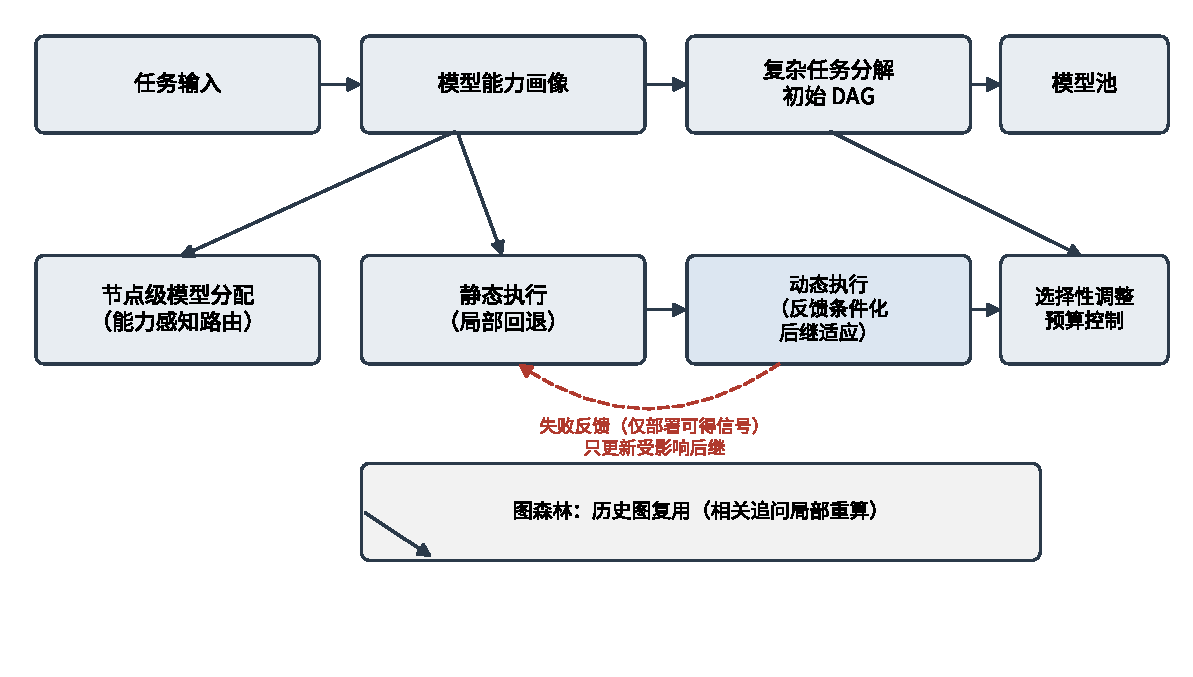
\includegraphics[width=0.95\textwidth]{fig_framework.pdf}
\caption{反馈感知自适应 DAG 路由整体框架。}
\label{fig:framework}
\end{figure}

\subsection{模型能力画像}

模型画像包含质量 $Q$、token 消耗 $C$ 与服务时长 $L$。区分条件能力与传播能力：对抽取模型 $e$ 与推理模型 $r$，
\begin{equation}
Q_{e,r}(x)=\mathbb{E}\!\left[Y\mid x,D,\operatorname{Extract}_e(D,x),r\right].
\end{equation}

\subsection{能力感知节点路由}

查询级选择 $r_q:x\to m$，节点级选择 $r_n:(x,\tau_i)\to m_i$。初始效用为
\begin{equation}
U(i,m)=\alpha\widehat{Q}(i,m)-\beta\widehat{C}(i,m)-\gamma\widehat{L}(i,m),\qquad
m_i^{*}=\arg\max_{m\in\mathcal{M}} U(i,m).
\end{equation}

\subsection{静态与动态执行}

静态模式按初始分配执行，节点失败时允许冻结的局部回退。动态模式定义为反馈条件化的后继适应：状态 $H_t$ 记录已执行模型、结果、失败经历与资源消耗，更新对象限于失败节点及其后代闭包 $A_t\cup \mathrm{Desc}_G(A_t)$。

\subsection{预算感知恢复与图森林}

剩余预算 $B_C^{\mathrm{rem}}=B_C-\sum_j c_j$。图森林 $F=\{G_1^{(\nu_1)},\dots,G_k^{(\nu_k)}\}$ 保存历史 DAG 与版本，支持相关追问的局部重算。

%======================================================================
\section{实验}\label{sec:exp}
%======================================================================

\subsection{实验设置}\label{sec:exp-setup}

实验以 MultiHiertt~\cite{zhao2022multihiertt} 财务表文推理为主，并以 TAT-QA~\cite{zhu2021tatqa}、MBPP~\cite{austin2021mbpp}（代码）与 Math500~\cite{hendrycks2021math,lightman2024verify}（数学）为跨域面板。模型池固定为 Qwen2.5-7B/14B/Coder-7B，生成配置 temperature 0、top\_p 1、max\_tokens 512，vLLM~\cite{kwon2023vllm} 推理。统计口径：任务级配对差值 $\Delta Q$、10000 次配对 bootstrap 95\% 区间与精确 McNemar 检验。

\subsection{阶段级模型能力异质性}\label{sec:exp-heterogeneity}

表~\ref{tab:node-quality} 显示三个候选模型在不同节点类型上的条件化质量与逐节点 Oracle 差距。

\begin{table}[htbp]
\centering\small
\caption{不同节点类型的条件化质量。}
\label{tab:node-quality}
\begin{tabular}{lccccc}
\toprule
类型 & 节点数 & medium & large & coder & 逐节点 Oracle \\
\midrule
抽取 & 193 & 0.3731 & 0.5959 & 0.3782 & 0.6943 \\
推理 & 100 & 0.3100 & 0.2500 & 0.3100 & 0.4100 \\
验证 & 200 & 0.5200 & 0.4550 & 0.5900 & 0.6200 \\
\bottomrule
\end{tabular}
\end{table}

\subsection{任务分解与能力解耦}\label{sec:exp-decomposition}

% 三臂分解基准（表 4-3/4-4/4-5）：拆分本身 −21.0pp 显著有害（TAT-QA），
% 异构分工 +5.0pp 但未完全抵消（31.7% vs 38.7%），复杂度单调 −27.1/+21.1/+50.0pp。
% 逐题分类：真分解 31 vs 接口 25；反事实 −8.5pp。
% 【迁移注记：完整表格与正文按冻结稿 §4.3 逐字填入】

\subsection{查询路由与节点路由}\label{sec:exp-routing}

% 表 4-6（+6.9pp，类型先验=节点路由）、表 4-7（两阶段路由 Conf-200/500 不显著）、表 4-8（风险—覆盖率）。
% 【迁移注记：按冻结稿 §4.4 填入】

\subsection{条件能力与传播能力差异}\label{sec:exp-propagation}

% 表 4-9（传播画像）、headroom 5.00/4.50/5.40/5.06pp。
% 【迁移注记：按冻结稿 §4.5 填入】

\subsection{跨模型组合与有限候选上界}\label{sec:exp-oracle}

% 表 4-10（3×3 矩阵）、表 4-11（Oracle 30.5%）。
% 【迁移注记：按冻结稿 §4.6 填入】

\subsection{静态与动态执行}\label{sec:exp-dynamic}

% 表 4-12（48 任务 +2.08pp ns）、250 确认 +2.8pp ns、
% 四节点面板表 4-13（Static 16.7% / Static-Matched 35.0% / Dynamic 36.7% / RealDetector 35.0%）。
% 归因：主要增益来自升级动作本身（+18.3pp），策略额外 +1.7pp ns。
% 【迁移注记：按冻结稿 §4.7 填入】

\subsection{故障诊断、恢复与预算}\label{sec:exp-recovery}

% 表 4-14（动作并集 8/116=6.9%）、表 4-15（预算响应）。
% 【迁移注记：按冻结稿 §4.8 填入】

\subsection{历史图复用}\label{sec:exp-graphforest}

% 20 追问、50% 调用减少、0/20 验证接受。辅助定位。
% 【迁移注记：按冻结稿 §4.9 填入】

\subsection{跨领域泛化与适用边界}\label{sec:exp-xdomain}

% 4.10.1 Math500 塌缩（54% vs 13–16%，双因素）；MBPP +6.0pp 支持性（p=0.070）；表 4-16。
% 4.10.2 外部基线（表 4-17）：RouteLLM-style 塌缩、cascade 反转、Self-Refine 85% vs 80% p=0.267。
% 4.10.3 三条件机制（图 5-1）：MBPP 降级 80→73、Math 盲区 62/67、先验反转。
% 【迁移注记：按冻结稿 §4.10 填入】

%======================================================================
\section{讨论}\label{sec:discussion}
%======================================================================

% 四问：5.1 分解非免费；5.2 条件≠传播；5.3 动态不创造能力；5.4 何时有效（三条件，图 5-1）。
% 【迁移注记：按冻结稿 §5 填入；图 5-1 以 fig_three_conditions.pdf 插入 5.4 末】

%======================================================================
\section{结论}\label{sec:conclusion}
%======================================================================

% 中心命题 + 三组证据 + 边界 + 未来方向（结构选择）。
% 【迁移注记：按冻结稿 §6 填入】

%======================================================================
% 参考文献
%======================================================================
\bibliographystyle{elsarticle-num}
\bibliography{references}

\end{document}
